% *********************************************************************
% © 2021–2024 Jeremy Sylvestre
%
% Permission is granted to copy, distribute and/or modify this document
% under the terms of the GNU Free Documentation License, Version 1.3 or
% any later version published by the Free Software Foundation; with no
% Invariant Sections, no Front-Cover Texts, and no Back-Cover Texts. A
% copy of the license is included in the appendix entitled “GNU Free
% Documentation License” that appears in the output document of this
% PreTeXt source code. All trademarks™ are the registered® marks of
% their respective owners.
%
% *********************************************************************

\newcommand*{\xmin}{-0.5}
\newcommand*{\xmax}{2.6}
\newcommand*{\ymin}{-2.5}
\newcommand*{\ymax}{12.5}

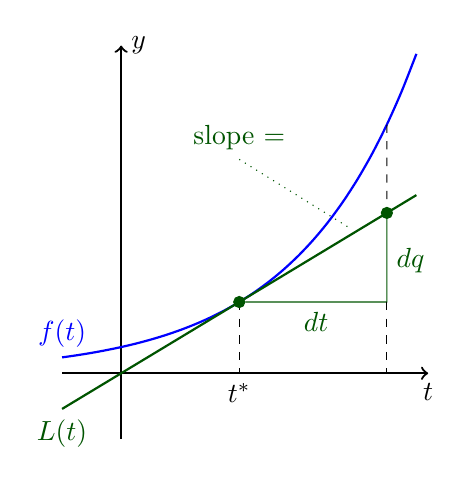
\begin{tikzpicture}
[
	yscale=0.333,
	xscale=1.5,
	closedpt/.style={circle,draw,fill,inner sep=0pt,minimum size=4pt},
]

	% axes
	\draw[->,thick] (\xmin,0) -- (\xmax,0) node[below] {$t$};
	\draw[->,thick] (0,\ymin) -- (0,\ymax) node[right] {$y$};

	% graphs

	% exp
	\draw[thick, blue, domain=2.5:-0.5, smooth] plot (\x,{exp \x}) node[above] {$f(t)$};

	% tangent
	\draw[thick,green!33!black] (2.5,6.796) -- (-0.5,-1.359) node[below] {$L(t)$};

	% base point
	\draw[dashed] (1,2.718) -- (1,0) node[below] {$t^\ast$};

	\node[closedpt,green!33!black] (base) at (1,2.718) {};
	\node[closedpt,green!33!black] (second) at (2.25,6.116) {};

	\draw[green!33!black] (base) to node[below] {$dt$} (2.25,2.718) to node[right] {$dq$} (second);

	\draw[dashed] (2.25,9.488) -- (second.north);
	\draw[dashed] (2.25,2.718) -- (2.25,0);

	\node[green!33!black] (tag) at (1,9) {slope $\displaystyle = \dqdt$};
	\draw[green!33!black,dotted] (tag.south) to (1.95,5.5);

\end{tikzpicture}
